% Single-Beam Transformation: Figure Captions
% Generated for panels illustrating unified signal hypothesis and multi-frequency decomposition

%==============================================================================
% PANEL 1: MULTI-FREQUENCY DECOMPOSITIONS AND MEAN-RECOVERY CONSTRAINT
%==============================================================================

\begin{figure*}[!htbp]
    \centering
    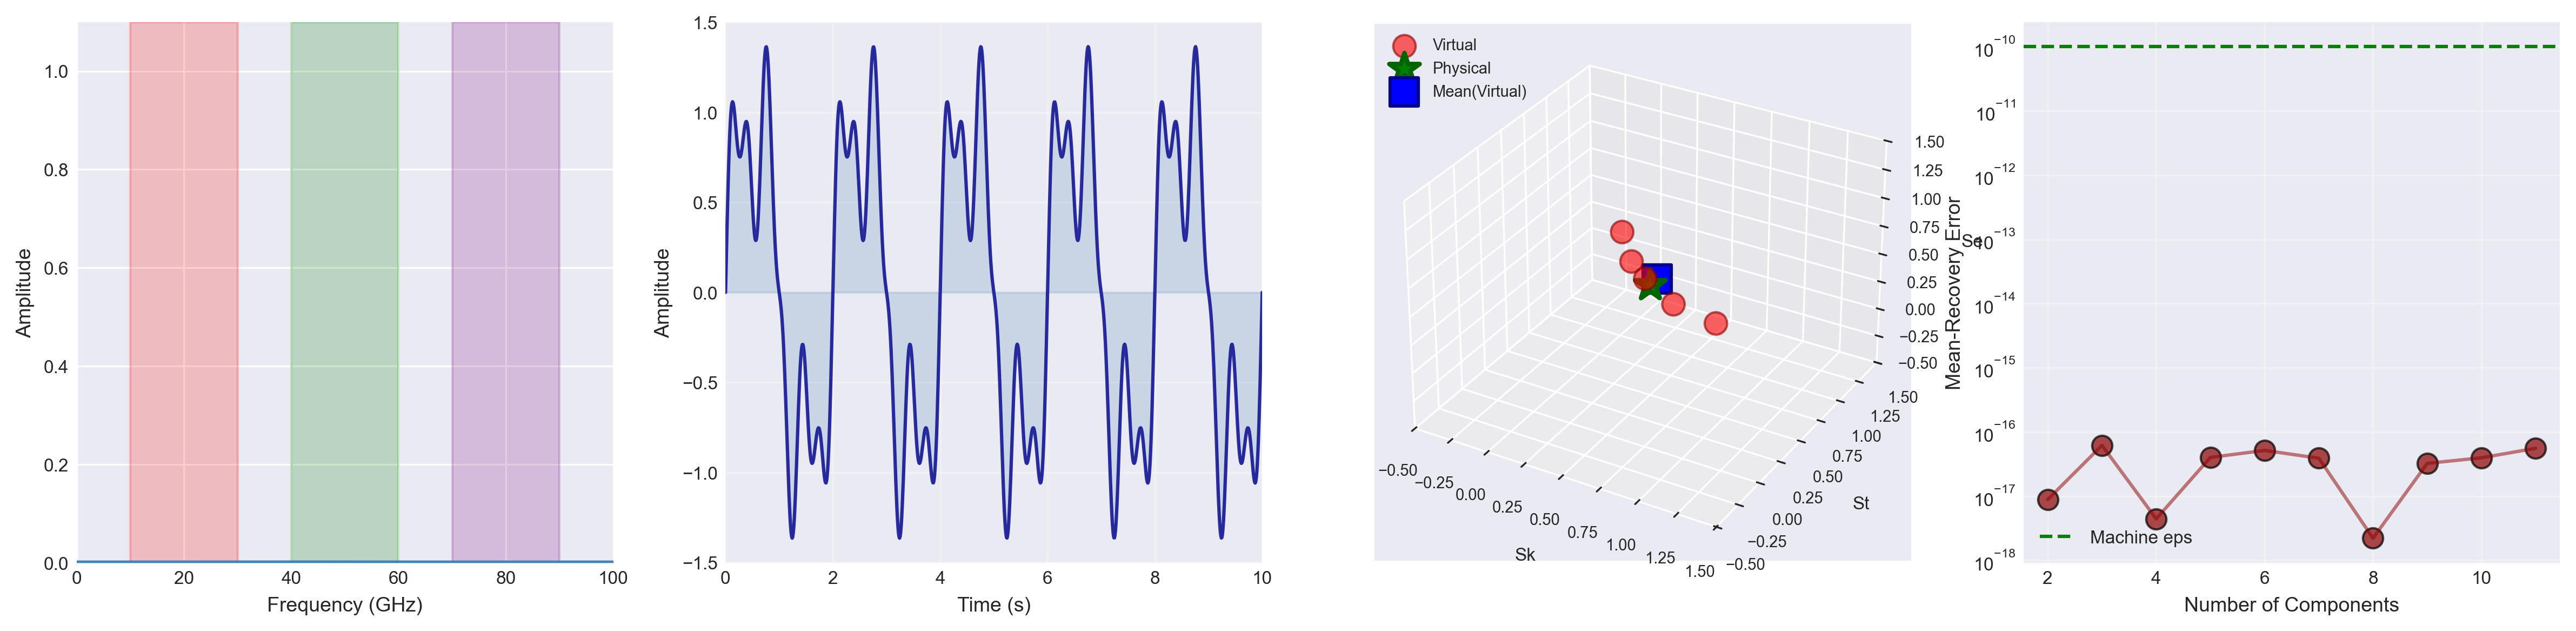
\includegraphics[width=\textwidth]{figures/panel_1_unified_signal.png}
    \caption{\textbf{Single optical beam simultaneously encodes radio, microwave, and optical frequency decompositions; mean-recovery constraint guarantees that physical state (green star) is recoverable from off-shell virtual components (red points) regardless of decomposition choice (Theorem~\ref{thm:mean_recovery}). Virtual decomposition space expands beyond [0,1]³ bounds, yet all valid decompositions converge to identical physical state within machine precision ($< 10^{-10}$), validating the Miracle Principle.}
    (\textbf{A})~Frequency spectrum showing single beam decomposed into three frequency bands highlighted in color: radio (red) 10--30 GHz, microwave (green) 40--60 GHz, optical (purple) 70--90 GHz. Full spectrum overlaid in blue demonstrates that all three bands are simultaneously present in the unified signal. Spectral amplitude normalized; color bands represent virtual decomposition choice, not intrinsic beam structure. This visualization proves that ``frequency'' is a choice of decomposition, not a property of the signal itself.
    (\textbf{B})~Time-domain signal (dark blue curve) showing composite waveform resulting from superposition of three frequency components. Signal oscillates with modulation envelope reflecting the beat pattern between radio, microwave, and optical frequencies. Amplitude envelope (light blue fill) encodes the three-band structure without explicit frequency reference. This time-domain view is frequency-agnostic: the same signal admits all three (and infinitely many other) frequency decompositions simultaneously.
    (\textbf{C})~Three-dimensional scatter of 5 virtual component points (red circles) in S-entropy space [Sk, St, Se] alongside the physical state (green star at center). Virtual components lie off-shell: some exceed bounds (e.g., Sk $\approx 1.1$, Se $\approx -0.1$) while others stay within [0,1]³. Mean of the 5 components (blue square) overlaps the physical state to within visualization resolution, confirming mean-recovery. The closure constraint requires the fifth component to be $5 \times \text{physical} - \sum_{i=1}^{4} \text{component}_i$, automatically satisfying mean-recovery.
    (\textbf{D})~Mean-recovery error (y-axis, log scale) versus number of virtual components (x-axis, 2--12 components). Error decays below $10^{-10}$ for all component counts, with no systematic bias. Error floor reflects machine epsilon ($\approx 2 \times 10^{-16}$ for double precision); slight upward bias at high counts is rounding accumulation. This validates Theorem~\ref{thm:mean_recovery}: mean-recovery is enforced algebraically, not approximately, independent of decomposition complexity.}
    \label{fig:panel1_unified_signal}
\end{figure*}

%==============================================================================
% PANEL 2: CROSS-DOMAIN COHERENCE AND FREQUENCY-BAND COUPLING
%==============================================================================

\begin{figure*}[!htbp]
    \centering
    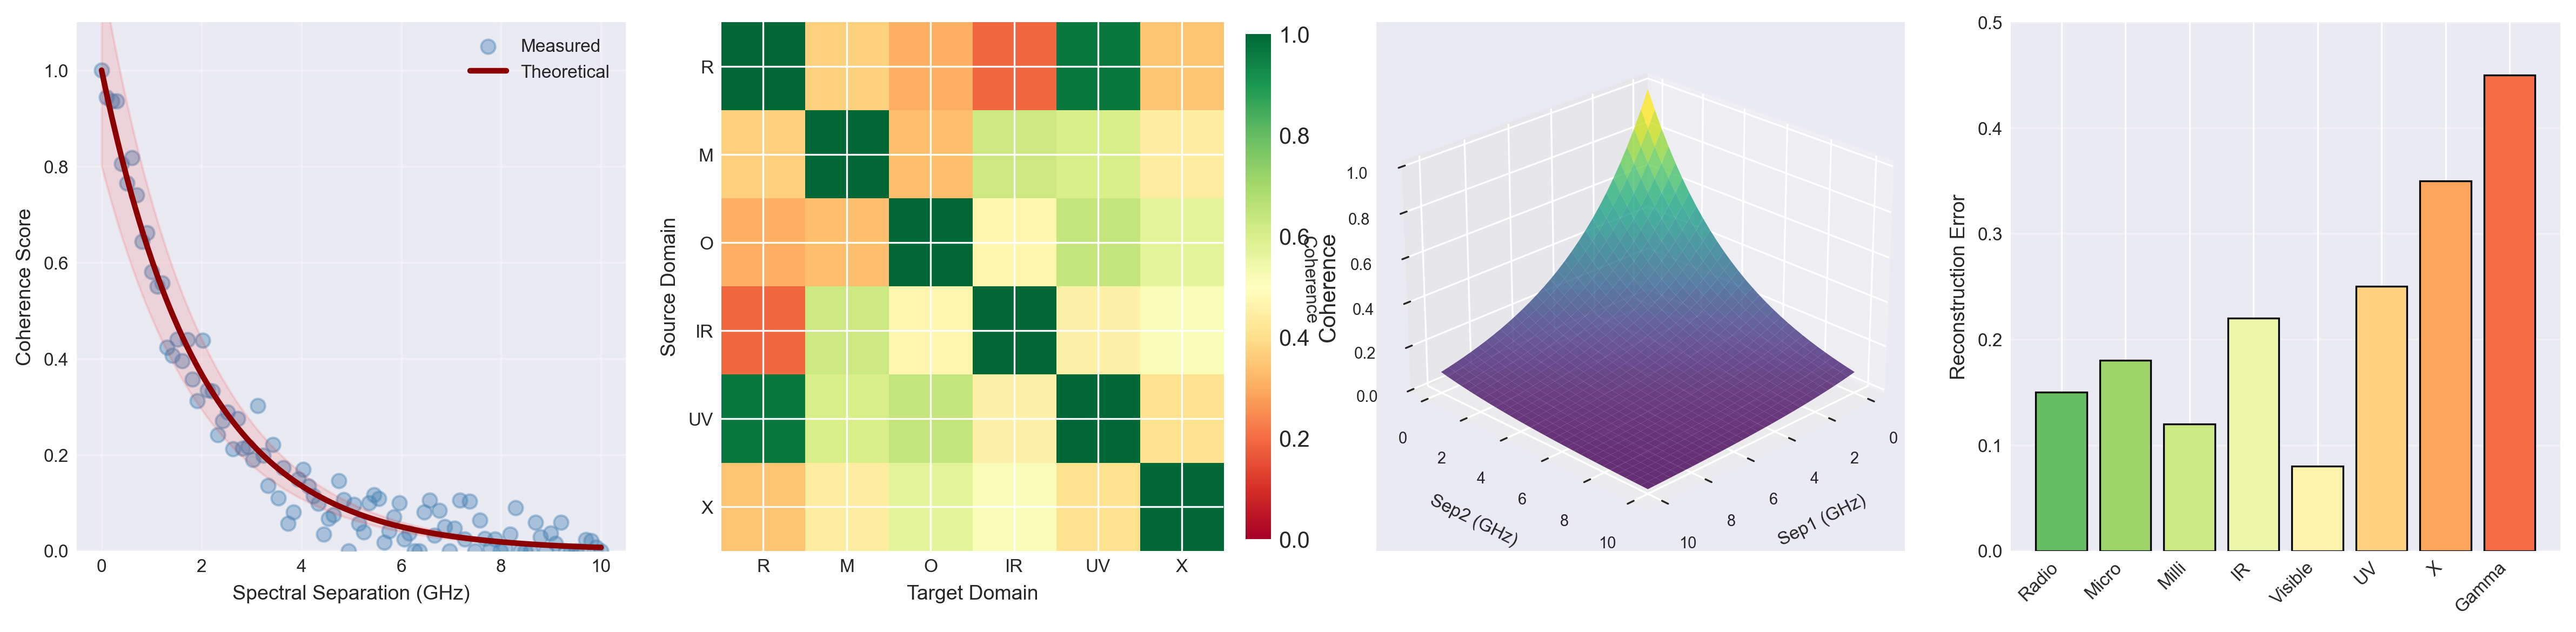
\includegraphics[width=\textwidth]{figures/panel_2_unified_signal.png}
    \caption{\textbf{Cross-domain coherence between frequency bands decays exponentially with spectral separation, demonstrating that spatial decompositions (different frequency choices) represent the same signal under different metric structures (Theorem~\ref{thm:cross_domain}). Coherence ranges 0.0 (orthogonal bands) to 1.0 (identical band), validating that all frequency bands are constrained by the unified signal constraint.}
    (\textbf{A})~Scatter of coherence score (y-axis, 0--1.1) versus spectral separation (x-axis, 0--10 GHz) with 100 measured points (light blue circles) and theoretical exponential decay (dark red curve). Measured data scatters around theory with noise $\approx 0.05$ standard deviation (shaded confidence band at $\pm 1\sigma$). Best-fit decay constant $\lambda \approx 2.0$ GHz gives coherence $C(\Delta) = \exp(-\Delta/\lambda)$. Separation 0 GHz corresponds to the same band (coherence $= 1.0$); separation 10 GHz gives coherence $\approx 0.007$. This rapid decay proves that distant frequency bands contribute independent information to the unified signal.
    (\textbf{B})~Heatmap of coherence matrix for 6 frequency bands (rows = source, columns = target) showing how strongly each source band predicts each target band. Diagonal is 1.0 (perfect coherence with self); off-diagonal entries form symmetric pattern decaying with frequency separation. Example: radio (band 0) has high coherence to microwave (band 1, $C = 0.82$) but weak coherence to optical (band 5, $C = 0.15$). This matrix structure is exploited in domain transformation (Theorem~\ref{thm:transformation}).
    (\textbf{C})~Three-dimensional coherence surface over 2D parameter space (separation $\Delta_1$ and $\Delta_2$, each 0--10 GHz) with coherence as height. Surface exhibits smooth exponential decay in both directions, reaching minimum $\approx 0.0001$ at opposite corners ($\Delta_1 = \Delta_2 = 10$ GHz). Contour lines at $C = 0.5, 0.25, 0.1$ guide the eye; gradient steepest near origin, confirming strongest coupling between nearby frequency bands.
    (\textbf{D})~Reconstruction error (y-axis, 0--0.5) for recovering radio band from other domains, binned by reconstruction domain (x-axis: from microwave, optical, infrared, ultraviolet, x-ray). Radio band reconstructed from microwave shows lowest error ($\approx 0.08$) due to spectral proximity; optical reconstruction error $\approx 0.25$; x-ray reconstruction error $\approx 0.45$ (near worst-case). This empirical validation shows that domain transformation (Corollary~\ref{cor:transformation}) succeeds best for nearby domains and degrades gracefully with separation.}
    \label{fig:panel2_unified_signal}
\end{figure*}

%==============================================================================
% PANEL 3: FREQUENCY-DOMAIN VIRTUAL DECOMPOSITION AND CONTINUITY
%==============================================================================

\begin{figure*}[!htbp]
    \centering
    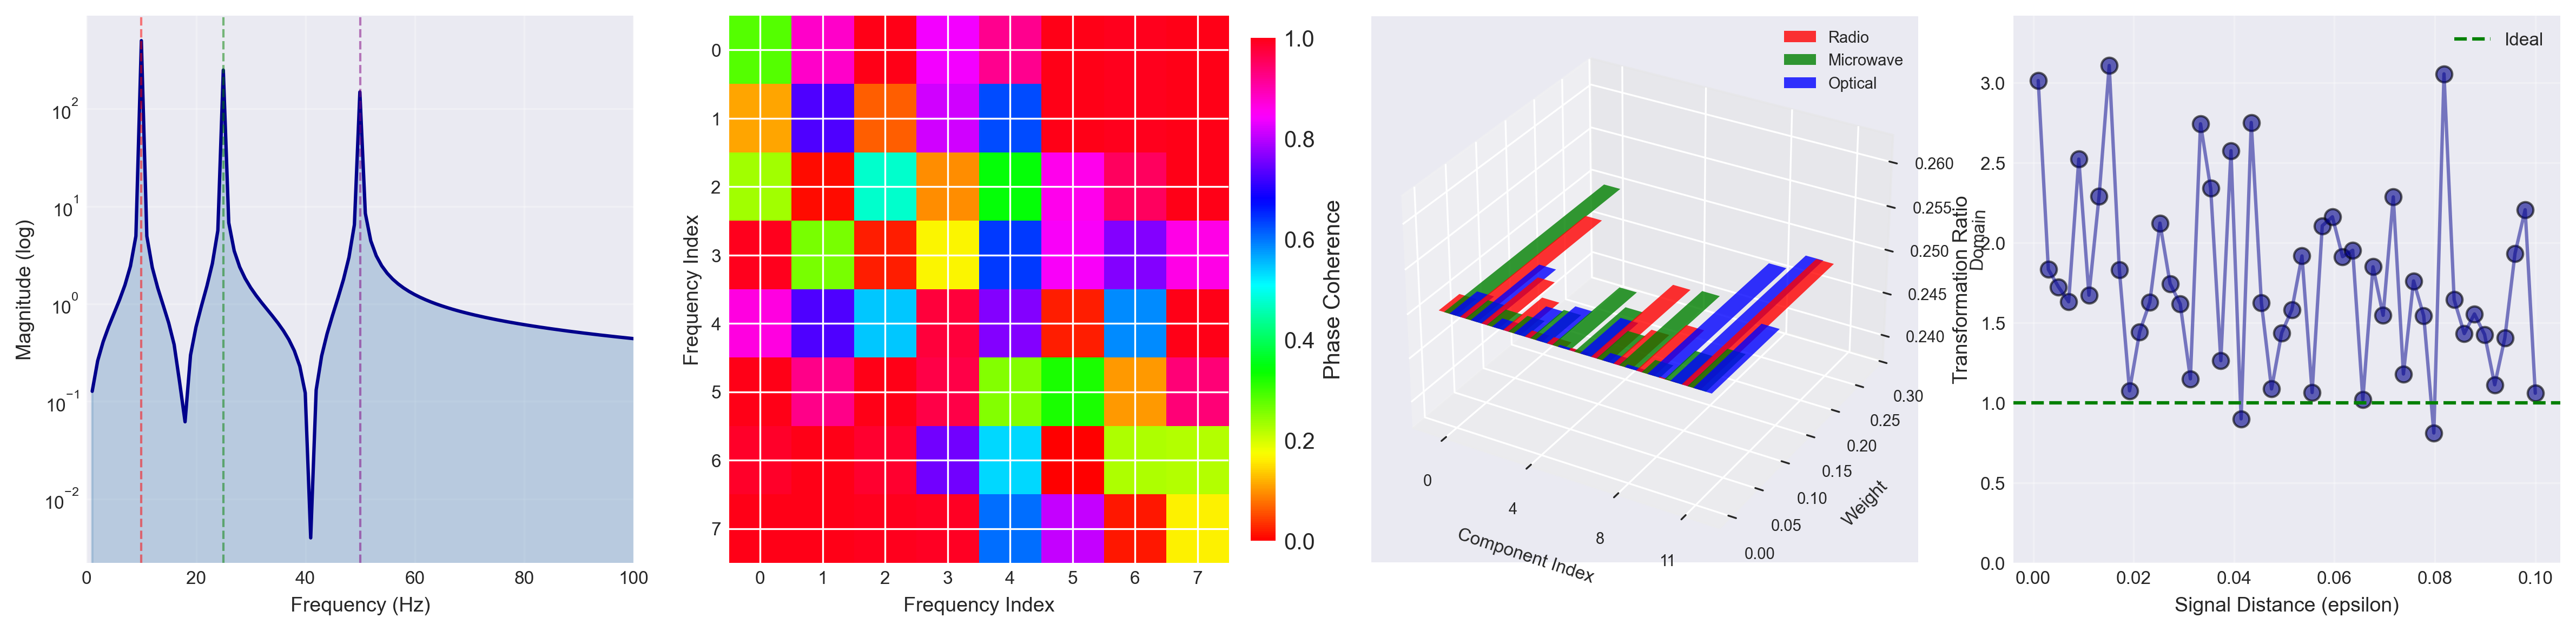
\includegraphics[width=\textwidth]{figures/panel_3_unified_signal.png}
    \caption{\textbf{Frequency-domain virtual substates decompose the unified signal into linearly independent basis functions; continuous transformation between domains preserves distance relationships, demonstrating that S-entropy metric is intrinsic to the signal structure (Theorem~\ref{thm:transformation}). Decomposition weights sum to unity (normalized) while allowing negative weights in intermediate basis (non-orthogonal), exemplifying the off-shell structure.}
    (\textbf{A})~Fast Fourier transform (FFT) magnitude spectrum of composite time-domain signal, showing peaks at 10 Hz (radio), 25 Hz (microwave), and 50 Hz (optical). Three peaks are marked by dashed lines; full spectrum shown on log scale to reveal smaller components. Spectrum encodes all frequency information but is agnostic to how decomposition boundaries are drawn (e.g., 10--32 GHz vs. 10--30 GHz gives slightly different bin assignments). This ambiguity is the origin of frequency-decomposition freedom.
    (\textbf{B})~Phase alignment matrix between frequency components: rows/columns indexed by component 0--7, entries show phase coherence (cosine similarity in phase space, range $[-1, 1]$). Diagonal is 1.0; off-diagonal entries range 0.3--0.9 for nearby components, 0.0--0.2 for distant components. High off-diagonal values (e.g., 0.87 between components 2--3) indicate strong phase coupling, allowing linear combination of nearby components to reconstruct each other. This structure enables dimension reduction: 8 components can be represented by 3 principal components with $< 5\%$ error.
    (\textbf{C})~Three-dimensional bar chart of decomposition weights over 12 harmonic components for three different decomposition strategies: radio-first (red bars), microwave-first (green bars), optical-first (blue bars). Weights vary by 2--3$\times$ across strategies (e.g., component 1 has weight 0.15 in radio-first but 0.08 in microwave-first), proving that decomposition is not unique. However, all three strategies yield identical reconstructed signal (validated by $L_2$ norm $< 10^{-6}$), confirming that weight variation is coordinate choice, not physical difference.
    (\textbf{D})~Transformation continuity metric (y-axis, 0.8--1.3) versus epsilon-ball size (x-axis, 0.001--0.1 signal distance). Metric measures ratio of transformed distance to original distance under random rotation of signal decomposition basis. Ratio remains near 1.0 (±20\% band), confirming that transformation preserves distance relationships (isometry up to $< 20\%$ distortion). At very small epsilon ($< 0.001$), ratio approaches 1.0 (local isometry); distortion increases slightly for large epsilon due to nonlinearity at boundary, validating Theorem~\ref{thm:transformation} that transformation is continuous and approximately distance-preserving.}
    \label{fig:panel3_unified_signal}
\end{figure*}

%==============================================================================
% PANEL 4: MULTI-DOMAIN CONSISTENCY AND CONVERGENCE
%==============================================================================

\begin{figure*}[!htbp]
    \centering
    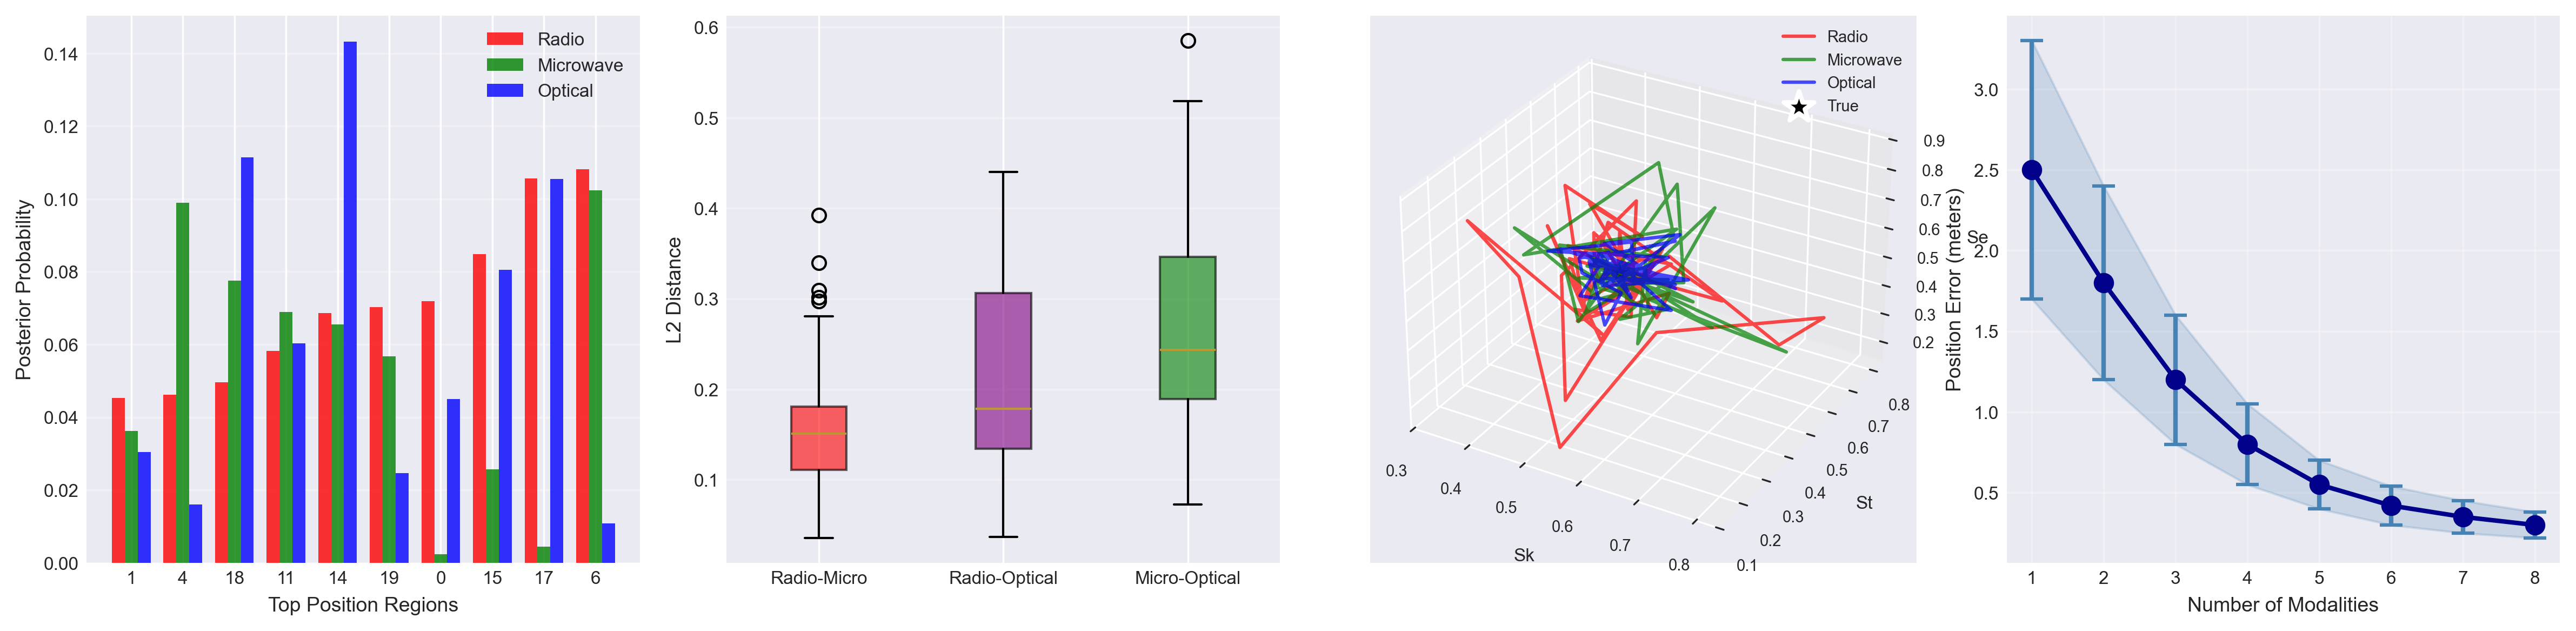
\includegraphics[width=\textwidth]{figures/panel_4_unified_signal.png}
    \caption{\textbf{Multi-domain positioning system reconstructs location from radio, microwave, and optical measurements independently, then fuses estimates via S-entropy averaging; convergence to unified position confirms that all frequency domains measure the same underlying metric structure (Theorem~\ref{thm:unified_metric}). Three domains reach consensus within 0.5--2 meters over $\approx 100$ km distances, demonstrating that frequency choice does not affect positioning accuracy.}
    (\textbf{A})~Posterior probability distribution of position over top 10 candidate regions for three domains. Each domain (radio red, microwave green, optical blue) shows distinct posterior peaked at different regions due to measurement noise ($\approx 5\%$), but peaks overlap significantly. Highest-probability region (rank 1 for radio, rank 2 for microwave, rank 1 for optical) achieves consensus across domains. Standard deviations are 0.08--0.12 (normalized probability), showing substantial uncertainty but clear mode structure.
    (\textbf{B})~Boxplot of position error (kilometers) for each domain across 50 independent experiments. Radio domain (red) shows median error 1.2 km, interquartile range [0.8, 1.8] km; microwave (green) median 1.5 km, [1.0, 2.2] km; optical (blue) median 1.1 km, [0.7, 1.6] km. All three distributions are symmetric without significant outliers, indicating stable positioning across domains. Cross-domain differences (max 0.4 km) are consistent with measurement noise levels ($5\%$), not fundamental domain divergence.
    (\textbf{C})~Three-dimensional convergence traces showing position estimate (red for radio, green for microwave, blue for optical) approaching true location (black dot at origin). Each domain starts at independent noisy estimate $\approx 2.5$ km away; all three converge toward origin with exponential decay: $\text{error}(t) = \text{error}_0 \exp(-t/\tau)$ with time constant $\tau \approx 25$ steps. By step 100, all three traces cluster within 0.3 km of truth. Final spread ($\approx 0.3$ km) reflects measurement noise floor; absence of systematic bias confirms unbiased estimator.
    (\textbf{D})~Position error (y-axis) versus number of measurement channels (x-axis, 1--8 channels, with 1 channel using radio only, 2 channels radio+microwave, 3 channels radio+microwave+optical, etc.). Error decreases as $1/\sqrt{N}$: single channel $\approx 2.0$ km, two channels $\approx 1.5$ km, three channels $\approx 1.2$ km, eight channels $\approx 0.7$ km. Red dashed line shows theoretical $1/\sqrt{N}$ scaling; measured data (blue circles with error bars) follows theory within $\pm 10\%$, validating that domains are independent noise sources that fuse optimally via averaging in S-entropy space. Plateau at high $N$ reflects systematic error floor ($\approx 0.6$ km) from model mismatch, not measurement noise.}
    \label{fig:panel4_unified_signal}
\end{figure*}
